%!TeX root=./maximo.tex

\section{Heap Cinético}
\label{heap:secao}
Um bom jeito de resolver o problema do máximo cinético é
manter uma fila de prioridades com os elementos da coleção.
Dessa maneira, o elemento que se encontra na raiz da fila
será o que possui o maior valor da coleção.
Para implementar a heap utilizaremos um vetor.

Inicialmente o vetor começa com os índices dos elementos
e construímos um heap de acordo com o valor de cada elemento
no instante $t = 0$, ou seja, com o valor $x_0$ de cada elemento.

Uma vez de posse do heap montado, construímos um certificado
para cada par $($filho, pai$)$ no heap. O $i$-ésimo certificado,
que se refere ao par das posições $i$ e $\floor{\dfrac{i}{2}}$,
consiste no instante de tempo em que o $i$-ésimo elemento
passará a ter um valor maior que o valor do
$\floor{\frac{i}{2}}$-ésimo elemento do vetor,
se esse instante for maior que o instante atual.
Do contrário, o certificado consiste em $+\infty$. % Esse valor do certificado é o seu \underline{prazo de validade}.

% Esses prazos de validade são os \underline{eventos} que causarão modificações no vetor que mantém os elementos ordenados pelo seu valor e consequentemente em alguns certificados.

Esses $n - 1$ certificados são colocados em uma fila de
prioridade $Q$, com o prazo de validade como chave. Estamos
interessados nos certificados com menor prazo de validade.

Para descrever a implementação das três operações, precisamos
estabelecer o nome das novas variáveis usadas. São elas:
\begin{enumerate}
    % \item $n$: o número de elementos dados;
    % \item $x_0$ e \textit{speed}: vetores com o valor e a velocidade inicial de cada um dos $n$ elementos;
    % \item \now: instante atual;
    \item \textit{heap}: vetor com os índices dos $n$ elementos
    formando um heap de acordo com o seu valor no instante
    \textit{now};
    \item \textit{cert}: vetor com os certificados, onde
    \textit{cert}$[i]$ guarda o certificado entre $i$ e
    $\floor{\dfrac{i}{2}}$, para $1 < i \leq n$.
    % \item \textit{Q}: fila de prioridade para os certificados.
\end{enumerate}

A interface da fila de prioridade que utilizaremos não se altera.

% Para implementar a operação updatePQ$(Q, i, t)$ em tempo logarítmico no número de elementos na fila de prioridade, é necessário utilizar um vetor adicional \textit{indQ} que guarda em \textit{indQ}$[i]$ a posição do $i$-ésimo certificado em $Q$.

Um evento está associado a um certificado $(i, t)$ que expira
no instante $t$. O tratamento do evento correspondente ao
certificado $(i, t)$ consiste em trocar de lugar os índices
armazenados nas posições $i$ e $\floor{\dfrac{i}{2}}$ do vetor
\heap, e recalcular o prazo de validade de até cinco certificados:
\begin{itemize}
    \item do $\floor{\frac{i}{2}}$-ésimo certificado, se $i > 1$;
    \item do $j$-ésimo certificado, se $i > 1$ e $j \leq n$,
    onde $j = 2\cdot \floor{\dfrac{i}{2}} + ((i + 1)\mod2)$
    é o irmão de $i$;
    \item do $(2i)$-ésimo certificado, se $2i \leq n$;
    \item do $(2i + 1)$-ésimo certificado, se $2i + 1 \leq n$.
\end{itemize}

O $i$-ésimo certificado também deve ser ajustado para $+\infty$.
Finalmente, é necessário fazer ajustes em $Q$, alterando a
chave dos certificados que sofreram alteração.

Novamente, na implementação da operação \textsc{event},
utilizaremos a rotina \textsc{update}$(i)$ que calcula a
nova validade $t$ do $i$-ésimo certificado, se $1 < i \leq n$,
e chama a rotina \textsc{updatePQ}$(Q, i, t)$.

\begin{algorithm}[H]
    \caption{Função \textsc{update}.} \label{max:update}
\begin{algorithmic}[1]
    \Function{update}{$i$}
        \If{$1 < i \leq n$}
            \State $t \leftarrow $
            \Call{expire}{$i,\floor{\frac{i}{2}}$}
            \State \Call{updatePQ}{$Q,i,t$}
        \EndIf
    \EndFunction
    % \LineComment{\Call{expire}{$i,j$} calcula a validade do certificado entre os elementos $i$ e $j$}
\end{algorithmic}
\end{algorithm}

\begin{algorithm}[H]
    \caption{Função \textsc{event}.} \label{max:evento}
\begin{algorithmic}[1]
    \Function{event}{}
        \State $i \leftarrow  $ \Call{minPQ}{$Q$}
        \While{\cert[$i$] = \now}
            \State \heap[$i$] $\leftrightarrow$
            \heap$[\floor{\frac{i}{2}}]$
            \State \Call{update}{$i$}
            \State \Call{update}{$\floor{\frac{i}{2}}$}
            \State \Call{update}{$2\cdot
            \floor{\frac{i}{2}} + ((i + 1)~mod~2)$}
            \State \Call{update}{$2i$}
            \State \Call{update}{$2i + 1$}
            \State $i \leftarrow  $ \Call{minPQ}{$Q$}
        \EndWhile
    \EndFunction
\end{algorithmic}
\end{algorithm}

\begin{figure}[H]
    \centering
    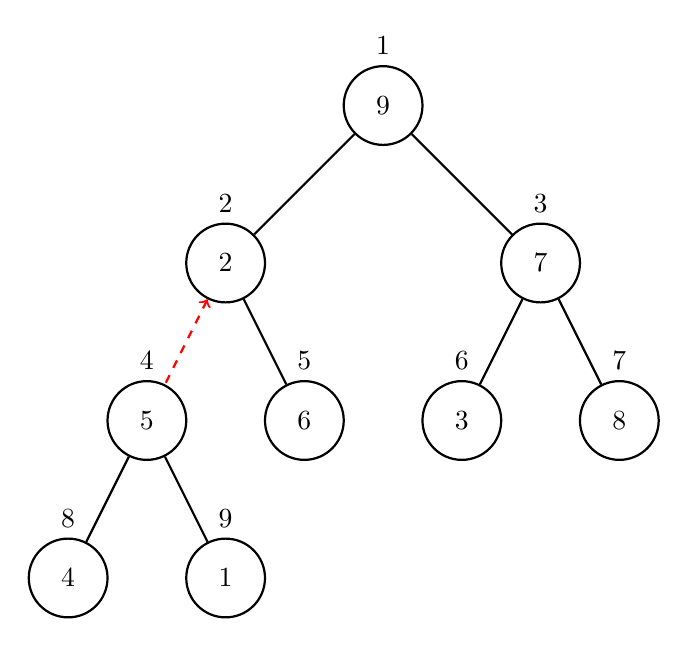
\begin{tikzpicture}[thick]
    \node[label={1},circle,draw,minimum size=1cm] (1) at (0,0) {$9$};
    \node[label={2},circle,draw,minimum size=1cm] (2) at (-2,-2) {$2$};
    \node[label={3},circle,draw,minimum size=1cm] (3) at (2,-2) {$7$};
    \node[label={4},circle,draw,minimum size=1cm] (4) at (-3,-4) {$5$};
    \node[label={5},circle,draw,minimum size=1cm] (5) at (-1,-4) {$6$};
    \node[label={6},circle,draw,minimum size=1cm] (6) at (1,-4) {$3$};
    \node[label={7},circle,draw,minimum size=1cm] (7) at (3,-4) {$8$};
    \node[label={8},circle,draw,minimum size=1cm] (8) at (-4,-6) {$4$};
    \node[label={9},circle,draw,minimum size=1cm] (9) at (-2,-6) {$1$};
        \tikzstyle{cert}=[<-, dashed, red]
        \draw[thick] (1) -- (2);
        \draw[thick] (1) -- (3);
        \draw[cert] (2) -- (4);
        \draw[thick] (2) -- (5);
        \draw[thick] (3) -- (6);
        \draw[thick] (3) -- (7);
        \draw[thick] (4) -- (8);
        \draw[thick] (4) -- (9);
        % \draw[->, color=red] (2) -- (3);
        % \draw[->] (3) -- (4);
        % \draw[->] (4) -- (5);
        % \draw[->] (1) edge (2) (2) edge (3) (3) edge (4) (4) edge (5)
    \end{tikzpicture}
    \caption{\cert[$4$] expirou.}
    \label{fig:maxdevent}
\end{figure}
\begin{figure}[H]
    \centering
    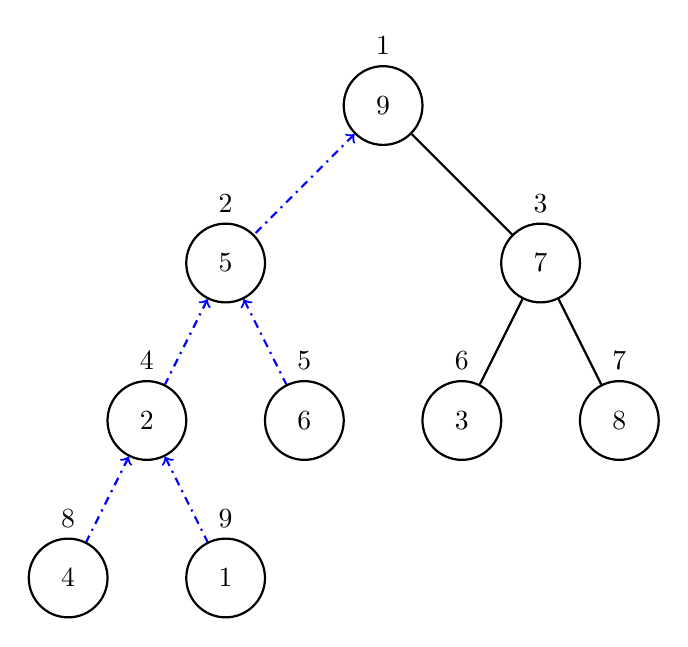
\begin{tikzpicture}[thick]
    \node[label={1},circle,draw,minimum size=1cm] (1) at (0,0) {$9$};
    \node[label={2},circle,draw,minimum size=1cm] (2) at (-2,-2) {$5$};
    \node[label={3},circle,draw,minimum size=1cm] (3) at (2,-2) {$7$};
    \node[label={4},circle,draw,minimum size=1cm] (4) at (-3,-4) {$2$};
    \node[label={5},circle,draw,minimum size=1cm] (5) at (-1,-4) {$6$};
    \node[label={6},circle,draw,minimum size=1cm] (6) at (1,-4) {$3$};
    \node[label={7},circle,draw,minimum size=1cm] (7) at (3,-4) {$8$};
    \node[label={8},circle,draw,minimum size=1cm] (8) at (-4,-6) {$4$};
    \node[label={9},circle,draw,minimum size=1cm] (9) at (-2,-6) {$1$};
        % \edef\pos{0}
        % \foreach \x in {1, 2,..., 5}{
        %     \pgfmathparse{\pos+2}
        %     \xdef\pos{\pgfmathresult}
        %     \node[circle,draw, minimum size=1cm] (\x) at  (\pos, 0) {$\x$};
        %     \node  at (\pos, -1) {$\x$};
        % }
        % \foreach \x [evaluate=\x as \y using int(\x + 1)] in {1, 2,..., 4}{
        %     \ifthenelse{\x==2}{\draw[->, draw=red] (\x) -- (\y);}{\draw[->, draw=black] (\x) -- (\y);}
        % }
        \tikzstyle{cert}=[<-, dashdotted, blue, thick]
        \draw[cert] (1) -- (2);
        \draw[thick] (1) -- (3);
        \draw[cert] (2) -- (4);
        \draw[cert] (2) -- (5);
        \draw[thick] (3) -- (6);
        \draw[thick] (3) -- (7);
        \draw[cert] (4) -- (8);
        \draw[cert] (4) -- (9);
        % \draw[->, color=red] (2) -- (3);
        % \draw[->] (3) -- (4);
        % \draw[->] (4) -- (5);
        % \draw[->] (1) edge (2) (2) edge (3) (3) edge (4) (4) edge (5)
    \end{tikzpicture}
    \caption{\heap[$4$] e \heap[$2$] foram trocados e \cert[$2$], \cert[$4$], \cert[$5$], \cert[$8$] e \cert[$9$] foram atualizados.}
    \label{fig:max:update}
\end{figure}

A operação \textsc{query\_max}$()$ consiste em devolver
\textit{heap}$[1]$, enquanto que a operação \textsc{change}$(j, v)$
consiste em alterar a posição $x_0[j]$ para
$x_0[j] + (\mathit{speed}[j] - v)\cdot now$,
a posição \textit{speed}[j] para \textit{v}
e recalcular os eventuais certificados de
que $j$ participa. Para tanto, a partir da
posição $i$ em que $j$ se encontra no vetor
\textit{heap}, podemos recalcular
\textit{cert}$[i]$ se $i > 1$, \textit{cert}$[2i]$ se
$2i \leq n$ e \textit{cert}$[2i + 1]$ se $2i + 1 \leq n$,
acionando a rotina \textsc{updatePQ} para fazer os devidos
acertos em $Q$ correspondentes a estas modificações.

\begin{algorithm}[H]
    \caption{Função \textsc{query\_max}.}
    \label{max:heap:query\_max}
\begin{algorithmic}[1]
    \Function{query\_max}{}
        \State \Return \heap$[1]$
    \EndFunction
\end{algorithmic}
\end{algorithm}

\begin{algorithm}[H]
    \caption{Função \textsc{change}.} \label{max:advance}
\begin{algorithmic}[1]
    \Function{change}{$j, v$}
        \State $x_0$[$j$] $\leftarrow x_0$[$j$]
        $+~($\speed[$j$] - $v)~\cdot~$\now;
        \State \speed[$j$] $\leftarrow v$
        \State \Call{update}{$i$}
        \State \Call{update}{$2i$}
        \State \Call{update}{$2i + 1$}
    \EndFunction
\end{algorithmic}
\end{algorithm}
\begin{figure}[H]
    \centering
    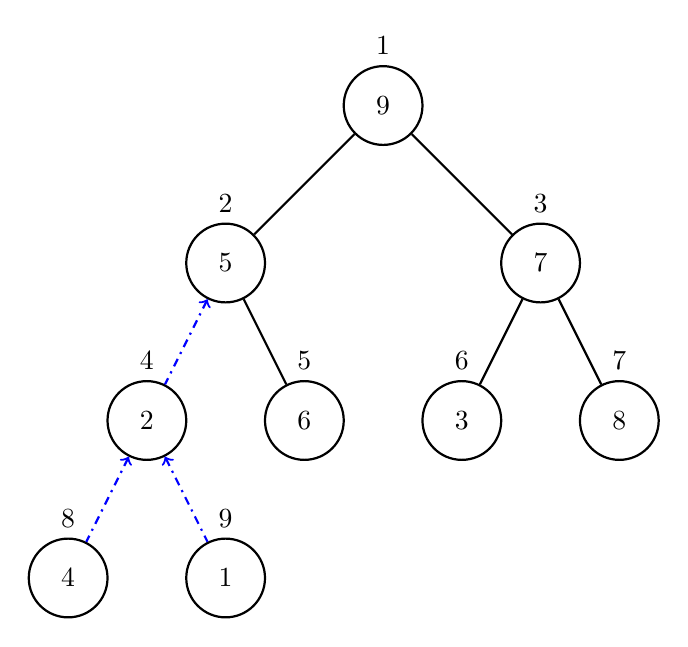
\begin{tikzpicture}[thick]
        \node[label={1},circle,draw,minimum size=1cm]
            (1) at (0,0) {$9$};
        \node[label={2},circle,draw,minimum size=1cm]
            (2) at (-2,-2) {$5$};
        \node[label={3},circle,draw,minimum size=1cm]
            (3) at (2,-2) {$7$};
        \node[label={4},circle,draw,minimum size=1cm]
            (4) at (-3,-4) {$2$};
        \node[label={5},circle,draw,minimum size=1cm]
            (5) at (-1,-4) {$6$};
        \node[label={6},circle,draw,minimum size=1cm]
            (6) at (1,-4) {$3$};
        \node[label={7},circle,draw,minimum size=1cm]
            (7) at (3,-4) {$8$};
        \node[label={8},circle,draw,minimum size=1cm]
            (8) at (-4,-6) {$4$};
        \node[label={9},circle,draw,minimum size=1cm]
            (9) at (-2,-6) {$1$};

        \tikzstyle{cert}=[<-, dashdotted, blue, thick]
        \draw[thick] (1) -- (2);
        \draw[thick] (1) -- (3);
        \draw[cert] (2) -- (4);
        \draw[thick] (2) -- (5);
        \draw[thick] (3) -- (6);
        \draw[thick] (3) -- (7);
        \draw[cert] (4) -- (8);
        \draw[cert] (4) -- (9);
    \end{tikzpicture}
    \caption{Após a mudança de velocidade do elemento 2,
    que se encontra em \heap[$4$], \cert[$4$], \cert[$8$] e
    \cert[$9$] foram atualizados.}
    \label{fig:predeventheap}
\end{figure}